\documentclass[letterpaper, 11pt]{article}
\usepackage[letterpaper, margin=1.4in]{geometry}
\usepackage{amsmath, amssymb}
\usepackage{graphicx}
\usepackage{verbatimbox}
\usepackage{listings}
\lstset{
 basicstyle=\ttfamily,
 columns=fullflexible,
 frame=single,
 breaklines=true,
}
\usepackage{caption}
\usepackage{subcaption}

\title{Pacman API Specification}
\author{Team Houston\\ Jonathan Wang, Manu Maheshwari, Yanjun Yang,\\ Tianqi Ma, Youyi Wei, Jiang Lin}
\date{}

\setlength\parindent{0pt}

\begin{document}
\maketitle
We use the command and strategy design patterns for this game. The character objects (such as Pacman and ghosts) act according to strategies, and use commands to act in the game. All game objects also use the observable-observer design pattern to receive updates about the game state and handle interactions.  

\section{Use Cases}
There are three groups of use cases for the Pacman game. We will look at the use cases and discuss how they will be handled by the API spec.
\begin{itemize}
  \item Game - overall game behavior
  \begin{itemize}
    \item display game objects - all game objects are observers stored in DispatchAdapter that will be passed to the view
    \item periodically spawn fruit - DispatchAdapter has a fruitTimer field that will determine when to add a fruit object to the observers
    \item track game values - DispatchAdapter has score and lives fields which will be updated during the game
  \end{itemize}
  \item Pacman - how Pacman interacts with the game
  \begin{itemize}
    \item move in all directions based on user input - Pacman moves by a update strategy. The direction can be changed by the /switchDirection request
    \item does not go through walls - Pacman has an interact strategy that will handle collisions
    \item warp through exits - Pacman has an interact strategy that will handle collisions
    \item eat food - Pacman has an interact strategy that will handle collisions
  \end{itemize}
  \item Ghosts - how ghosts interact with the game
  \begin{itemize}
    \item move based on strategy - ghosts each have an update strategy
    \item does not go through walls - ghosts have an interact strategy that will handle collisions
    \item warp through exits - ghosts have an interact strategy that will handle collisions
    \item eat Pacman - ghosts have an interact strategy that will handle collisions
    \item eaten by Pacman when afraid - DispatchAdapter has an afraidTimer field that tracks when ghosts can be eaten by Pacman. The actual ghost-Pacman interaction is handled by the interact strategy
    \item go to jail - ghosts each have a jailTimer that tracks how long they stay in jail for 
  \end{itemize}
\end{itemize}

\section{View}
We have a single canvas in index.html where the game and game values will be displayed. In view.js there are functions to start and run the game and display game objects. The view makes requests to the controller to reset the game as well as update the game state. 

\begin{itemize}
  \item /resetGame - called on page load to setup the game
  \item /updateGame - called every 0.1 sec to receive game state. Game objects are drawn onto the canvas based on received data
  \item /switchDirection - called based on user input to change Pacman direction
\end{itemize}

Based on the returned data, the view draws the game objects onto the canvas. The ghosts and fruit are image files, and the remaining game objects are drawn using canvas functions. Display-only features that do not affect the game operation, such as flashing ghosts, blinking dots, and the Pacman animation are handled exclusively in the view.

\section{Controller}
The PacWorldController processes GET and POST requests and returns the JSON representation of the DispatchAdapter, which contains all the game objects in the PacWorld. The controller creates the DispatchAdapter and defines the REST endpoints \\ 

These are the supported requests handled by PacWorldController:
\begin{itemize}
  \item /resetGame - gets the canvas dimension and passes it to the DispatchAdapter; resets game values and resets all game objects to the starting positions
  \item /udpateGame - updates the game state with collisions, new locations, removed objects, etc.
  \item /switchDirection - takes user input to change the Pacman movement direction
\end{itemize}

The controller also gets and sets the port assigned by Heroku for hosting.

\section{Model}
The model includes the DispatchAdapter, commands, strategies, and game objects.

\subsection{DispatchAdapter}
The DispatchAdapter communicates with the model and the view. It contains the observers and values for the game. These values include:
\begin{itemize}
  \item Point dims - dimensions of game map
  \item static int gridSize - size of grid spaces for game scaling (static for easy access in concrete classes)
  \item int score - current game score
  \item int lives - current Pacman lives
  \item int fruitTimer - cool down timer for fruit spawning
  \item int afraidTimer - time that Pacman can eat ghosts 
\end{itemize}

Methods in the DispatchAdapter include getters and setters for the fields as well as methods to run the game.
\begin{itemize}
  \item DispatchAdapter() - constructor
  \item initializeMap() - return 2D array representing layout of game objects
  \item initializeGame() - reset observers and game values and add game objects according to map layout
  \item updatePacWorld() - update game state, handling object movement and collisions
  \item switchDirection(String body) - read user input from body and change Pacman direction
 \end{itemize}
 
\subsection{Command}
The cmd package has an interface IGameObjectCmd.
\begin{itemize}
  \item IGameObjectCmd - interface for all commands to allow game objects to act on game. The concrete commands will be UpdateCmd (object update), CollisionCmd (object collision), and SwitchCmd (Pacman direction). These three tasks can be performed with just the execute() method defined in the interface. 
  \begin{itemize}
    \item execute(AGameObject context) - allows context to act on the game state. The context object is the receiver that executes the command.
  \end{itemize}
\end{itemize}

\subsection{Strategy}
The strategy package has two interfaces - IUpdateStrategy and IInteractStrategy. 
\begin{itemize}
  \item IUpdateStrategy - interface for strategies that update individual game objects. Pacman will have a single update strategy that lets it move based on the user-specified direction. Ghosts will each have an update strategy for attacking and all use the same strategy when fleeing. No other game object has an update strategy, besides a null strategy.
  \begin{itemize}
    \item getName() - return update strategy name
    \item update(AGameObject context) - updates the state of the context object
  \end{itemize}  
  \item IInteractStrategy - interface for strategies that handle interaction between objects. All interactions in the game occur between two objects of different types. All interactions between two objects will be handled by one object. For instance, everything that occurs between Pacman and ghosts is handled by ghosts, and Pacman does not handle that interaction at all. This simplifies the number of cases to track and reduces the need for switching interaction strategies.
  \begin{itemize}
    \item getName() - return interact strategy name
    \item interact(AGameObject src, AGameObject dest) - handles interaction between src and dest objects
  \end{itemize}
\end{itemize}

\subsection{Game Objects}
The gameobject package has an abstract class AGameObject. Two abstract classes, ACharater and AFood, extend AGameObject. The abstract classes and the concrete classes are shown in figure \ref{fig1}. 

\begin{figure}[htbp] 
  \centering
  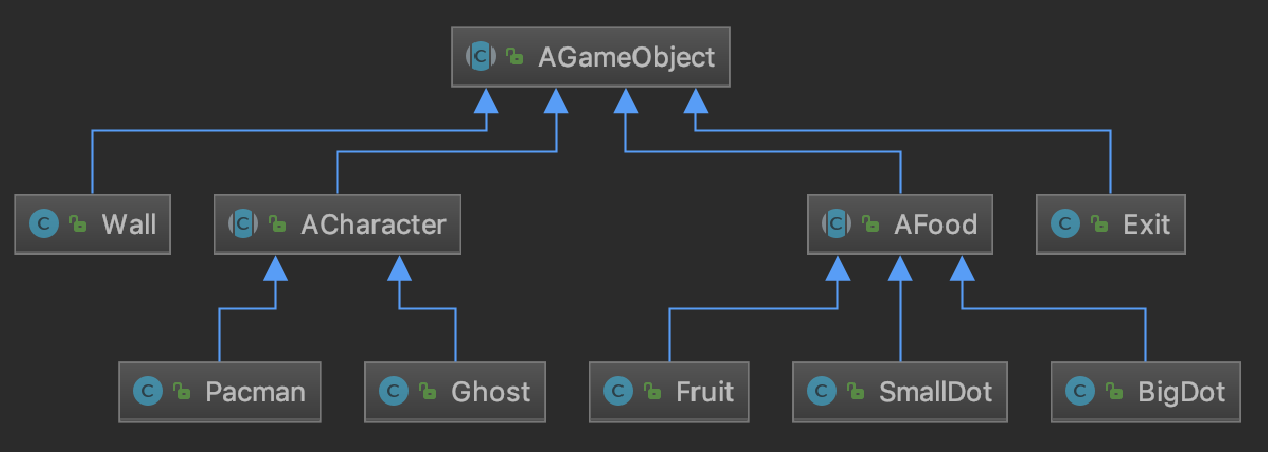
\includegraphics[width=.85\linewidth]{objects.png} 
  \caption{Game Objects}
  \label{fig1} 
\end{figure}

Several of the abstract and concrete classes do not have additional fields or methods from their parent class, but having the added class hierarchy simplifies object creation, and allows for extensible behavior. Each concrete class constructor sets the object size based on the DispatchAdapter gridSize. This allows for easy scalability with just one variable change.

\begin{itemize}
  \item AGameObject - all game objects have a location, type, and size
  \begin{itemize}
    \item AGameObject(Point location, String type, int size) - constructor
    \item update(Observable obs, Object o) - update game object by executing o as a command
  \end{itemize}
  \item ACharacter - all characters extend AGameObject and have a velocity, updateStrategy, and interactStrategy
  \begin{itemize}
    \item ACharacter(Point loc, String type, Point vel, IUpdateStrategy updateStrategy, IInteractStrategy interactStrategy, int size) - constructor
    \item collision(AGameObject gameObject) - handle collision against gameObject
  \end{itemize}
  \item AFood - all food extends AGameObject. This abstraction layer is used for easier collision checking and possible extensibility, if new behaviors are added for food objects.
\end{itemize}

\end{document}